\documentclass{article}
\usepackage[T1]{fontenc}
\usepackage{lmodern}
\usepackage{graphicx}
\usepackage{amsmath,amssymb}
\usepackage[a4paper,margin=2cm]{geometry}
\usepackage[absolute,overlay]{textpos}
\setlength{\TPHorizModule}{1mm}
\setlength{\TPVertModule}{1mm}
\usepackage[indonesian]{babel}
\usepackage{hyperref}
\setlength{\emergencystretch}{2em}
% unit: Halaman 24

\begin{document}

% === Halaman 24 (python/native) ===

• Luaran proses substitusi adalah blok B yang 

panjangnya 32 bit. 

• Blok B menjadi masukan untuk proses permutasi. 

• Tujuan permutasi adalah untuk mengacak hasil 

proses substitusi kotak-S. 

• Permutasi dilakukan dengan menggunakan 

matriks permutasi P (P-box) sbb:

16 

7 

20 

21 

29 

12 

28 

17 

1 

15 

23 

26 

5 

8 

31 

10 

2 

8 

24 

14 

32 

27 

3 

9 

19 

13 

30 

6 

22 

11 

4 

25 


24

% deskripsi: gambar native xref 116
\noindent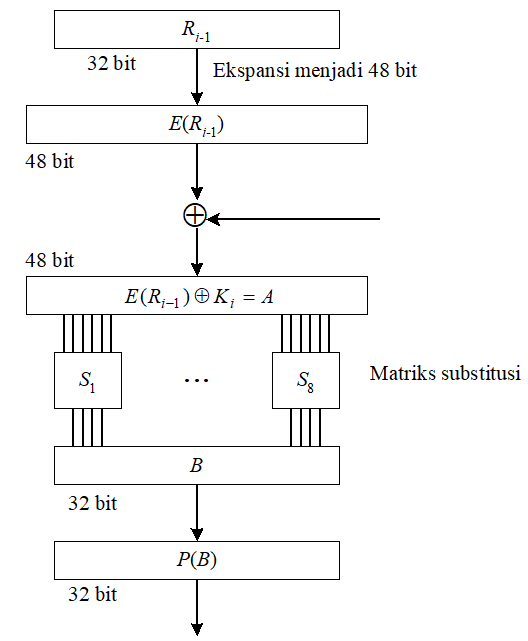
\includegraphics[width=0.85\textwidth]{../../images/python/page_024_img_01.png}

\end{document}
